\documentclass[11pt, oneside]{article}   	% use "amsart" instead of "article" for AMSLaTeX format
\usepackage{geometry}                		% See geometry.pdf to learn the layout options. There are lots.
\geometry{letterpaper}                   		% ... or a4paper or a5paper or ... 
%\geometry{landscape}                		% Activate for for rotated page geometry
%\usepackage[parfill]{parskip}    		% Activate to begin paragraphs with an empty line rather than an indent
\usepackage{graphicx}				% Use pdf, png, jpg, or eps� with pdflatex; use eps in DVI mode
								% TeX will automatically convert eps --> pdf in pdflatex		
\usepackage{amssymb}
\usepackage{amsmath}
\usepackage{parskip}
\usepackage{color}

\title{Inverse}
%\author{The Author}
%\section{}
% \subsection*{R code}
\date{}							% Activate to display a given date or no date

\graphicspath{{/Users/telliott_admin/Dropbox/Tex/png/}}

% \begin{center} 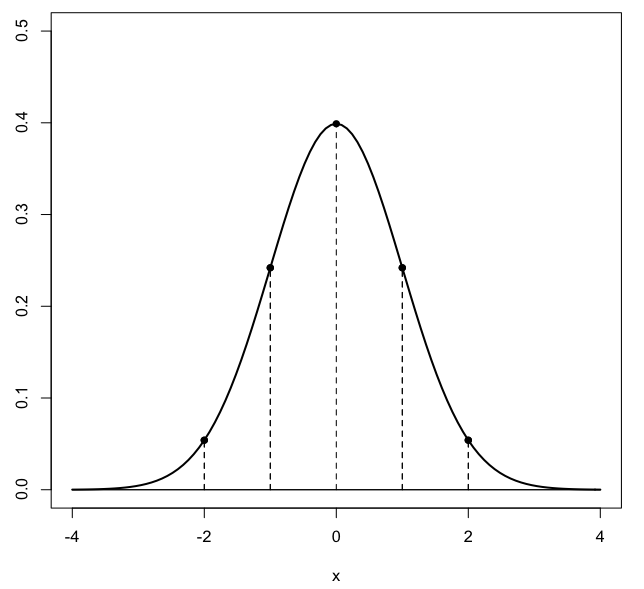
\includegraphics [scale=0.4] {gauss3.png} \end{center}
% \begin{bmatrix} a  &  b \\ c  &  d \end{bmatrix}
% \bigg |_

\begin{document}
\maketitle
\large

This short write-up discusses the matrix inverse.  Consider a basic matrix equation such as 

\[ A \mathbf{x} = \mathbf{b} \]

where $A$ is a $2 \times 2$ matrix, and $\mathbf{b}$ is a \emph{known} vector of size $2$, while $\mathbf{x}$ is a vector of \emph{unknowns}.  

In other words, the above is shorthand for

\[
\begin{bmatrix}
a_{11} & a_{12} \\
a_{21} & a_{22}
 \end{bmatrix}
\
\begin{bmatrix}
x \\
y
 \end{bmatrix}
=
\begin{bmatrix}
b_1 \\
b_2
 \end{bmatrix}
 \]
 
 Which can in turn be written as two simultaneous linear equations
 
\[ a_{11} x +  a_{12} y = b_1 \]
\[ a_{21} x +  a_{22} y = b_2 \]

There are several ways to solve a system like this one.  One method is Gaussian elimination.  A second way is to find the inverse of the matrix $A$.  The inverse has the notation $A^{-1}$ and it is defined by this property

\[ A A^{-1}= I = A^{-1} A \]
where $I$ is the identity matrix
\[ I = 
\begin{bmatrix}
1 & 0 \\
0 & 1
 \end{bmatrix}
\]
Since
\[ I \mathbf{x} = \mathbf{x} \]
in other words
\[ 
\begin{bmatrix}
1 & 0 \\
0 & 1
 \end{bmatrix}
\begin{bmatrix}
x \\
y
 \end{bmatrix}
=
\begin{bmatrix}
x \\
y
 \end{bmatrix}
 \]
it should be clear that if we multiply our original equation on both sides by $A^{-1}$
\[ A^{-1} A \mathbf{x} = \mathbf{x} =  A^{-1} \mathbf{b} \]
the left-hand side has become just $\mathbf{x}$, which is our unknown, while we know how to compute $A^{-1} \mathbf{b}$, given $A^{-1}$.

\subsection*{finding the inverse}

For this part I want to switch symbols:

\[
A =
\begin{bmatrix}
a & b \\
c & d
 \end{bmatrix},
 \ \ \
A^{-1}  =
\begin{bmatrix}
e & f \\
g & h
 \end{bmatrix}
\]
We know $abcd$ and we need to find $efgh$.
The result we want is $A \times A^{-1} = I$
\[
\begin{bmatrix}
a & b \\
c & d
 \end{bmatrix}
 \times
\begin{bmatrix}
e & f \\
g & h
 \end{bmatrix}
 =
\begin{bmatrix}
1 & 0 \\
0 & 1
 \end{bmatrix}
\]
We have four equations, but if you write them out you'll see it looks like a bit of a mess!  Luckily, I know an easy formula for the $2 \times 2$ case:

\[
A^{-1}  = \frac{1}{|A|} 
\begin{bmatrix}
d & -b \\
-c & a
 \end{bmatrix}
=
\frac{1}{ad-bc} 
\begin{bmatrix}
d & -b \\
-c & a
 \end{bmatrix}
\]

We switch $a$ and $d$, negate $b$ and $c$, and multiply by $1$ over the determinant of $A$.  I claim that

\[
A^{-1} A = 
\frac{1}{ad-bc} 
\begin{bmatrix}
d & -b \\
-c & a
 \end{bmatrix}
\begin{bmatrix}
a & b \\
c & d
 \end{bmatrix}
= I =
\begin{bmatrix}
1 & 0 \\
0 & 1
 \end{bmatrix}
\]

I think it is clear by inspection that this is correct.  For example, the first term is $1/(ad-bc) \times (ad - bc) = 1$.

There are many other formulas for finding the inverse (see wikipedia).  A standard approach is to go through the steps of Gaussian elimination to convert $A$ to $I$.  These can be represented as a series of matrix multiplications.  As an example, suppose we have

\[ A = 
\begin{bmatrix}
1 & -1 \\
2 & 2
 \end{bmatrix}
\]

The steps of Gaussian elimination (all the way to I) generate in turn

\[ 
\begin{bmatrix}
1 & -1 \\
2 & 2
 \end{bmatrix}
 \rightarrow
\begin{bmatrix}
1 & -1 \\
0 & 4
 \end{bmatrix}
 \rightarrow
\begin{bmatrix}
1 & 0 \\
0 & 4
 \end{bmatrix}
 \rightarrow
\begin{bmatrix}
1 & 0 \\
0 & 1
 \end{bmatrix}
\]

The matrix multiplications that do this are:

\[ 
E_1 = 
\begin{bmatrix}
1 & 0 \\
-2 & 1
 \end{bmatrix}
\]
\[
E_1 A = 
\begin{bmatrix}
1 & 0 \\
-2 & 1
 \end{bmatrix}
\times
\begin{bmatrix}
1 & -1 \\
2 & 2
 \end{bmatrix}
 =
\begin{bmatrix}
1 & -1 \\
0 & 4
 \end{bmatrix}
\]

\[ E_2 =
\begin{bmatrix}
1 & 1/4 \\
0 & 1
 \end{bmatrix}
\]
\[ 
E_2(E_1 A) = 
\begin{bmatrix}
1 & 1/4 \\
0 & 1
 \end{bmatrix}
\times
\begin{bmatrix}
1 & -1 \\
0 & 4
 \end{bmatrix}
 =
\begin{bmatrix}
1 & 0 \\
0 & 4
 \end{bmatrix}
\]

\[ E_3 =
\begin{bmatrix}
1 & 0 \\
0 & 1/4
 \end{bmatrix}
\]
\[
E_3(E_2(E_1 A))) =
\begin{bmatrix}
1 & 0 \\
0 & 1/4
 \end{bmatrix}
\times
\begin{bmatrix}
1 & 0 \\
0 & 4
 \end{bmatrix}
 =
\begin{bmatrix}
1 & 0 \\
0 & 1
 \end{bmatrix}
 =
 I
\]
Putting it all together
\[ E_3 \times E_2 \times E_1 \times A = I \]
Therefore
\[ E_3 \times E_2 \times E_1 = A^{-1} \]
\[ E_3 \times E_2 \times E_1 = 
\begin{bmatrix}
1 & 0 \\
0 & 1/4
\end{bmatrix}
\begin{bmatrix}
1 & 1/4 \\
0 & 1
 \end{bmatrix}
\begin{bmatrix}
1 & 0 \\
-2 & 1
 \end{bmatrix}
=
\begin{bmatrix}
1 & 1/4 \\
0 & 1/4
 \end{bmatrix}
\begin{bmatrix}
1 & 0 \\
-2 & 1
 \end{bmatrix}
=
\begin{bmatrix}
1/2 & 1/4 \\
-1/2 & 1/4
 \end{bmatrix}
 = \frac{1}{4}
\begin{bmatrix}
2 & 1 \\
-2 & 1
 \end{bmatrix}
\]
If you remember the rule for $2 \times 2$ from above, you'll see that we did indeed switch $a$ with $d$, negate $b$ and $c$, and multiply by $1/det(A)$.





\end{document}  